\documentclass[
    10pt,
    pdf,
    UTF8,
    aspectratio=169
]{beamer}

% font settings
%% English fonts
% \usefonttheme{serif}
% \usepackage{times}
%% math fonts
\usefonttheme{professionalfonts}

% shape
% shape
% more details, see % https://zhuanlan.zhihu.com/p/138021900
\setbeamertemplate{section in toc}[square]
\setbeamertemplate{subsection in toc}[square]

\setbeamertemplate{enumerate subitem}{\arabic{enumi}}
\setbeamertemplate{enumerate subitem}{\alph{enumii}}
\setbeamertemplate{enumerate subsubitem}{\roman{enumiii}}
\setbeamertemplate{itemize item}[square]
\setbeamertemplate{itemize subitem}[triangle]
\setbeamertemplate{itemize subsubitem}[circle]
\setbeamertemplate{blocks}[rounded][shadow=true]
% TODO
% \setbeamertemplate{title page}[rounded][shadow=true]
\setbeamertemplate{footline}[frame number]
\setbeamertemplate{caption}[numbered]
% TODO can't work
% \setbeamertemplate{caption}{\insertcaptionnumber sd \insertcaptionname}

% color
% color
% https://zhuanlan.zhihu.com/p/137877025
\definecolor{ScutColor1}{RGB}{0, 70, 144}
\definecolor{ScutColor2}{RGB}{0, 110, 180}
\definecolor{ScutColor3}{RGB}{100, 150, 200}
\setbeamercolor{structure}{fg=ScutColor1} % witout bg=white

\setbeamercolor{title}{fg=white,bg=ScutColor1}
\setbeamercolor{section in toc}{fg=ScutColor1, bg=white}
\setbeamercolor{subsection in toc}{fg=ScutColor2, bg=white}
\setbeamercolor{block title}{fg=white, bg=ScutColor2}
\setbeamercolor{block body}{fg=black,bg=gray!10}
\setbeamercolor{block title alerted}{fg=white,bg=red!75!black}
\setbeamercolor{block body alerted}{fg=black,bg=red!5}
\setbeamercolor{block title example}{fg=white,bg=green!50!black}

% package
% figure
\usepackage{graphicx}
\usepackage[]{subfig}
\usepackage{tikz}

% layout
\usepackage{multicol}
\usepackage{multirow}

% code
\usepackage{minted}
% Algorithm
%% Float of algorithm
\usepackage{algorithm}
%% Body of algorithm
\usepackage{algorithmic}
%% Custom setting for algorithmic
\renewcommand{\algorithmicrequire}{\textbf{Input:}} 
\renewcommand{\algorithmicensure}{\textbf{Output:}}

% reference
\usepackage[style=ieee]{biblatex}
\addbibresource{ref.bib}
\usepackage{hyperref}

% math
%% package for math
\usepackage{amssymb,amsmath}
\newcommand{\vect}[1]{\boldsymbol{#1}} % vector
\newcommand{\mat}[1]{\mathbf{#1}}      % matrix
\newcommand{\tensor}[1]{\mathsf{#1}}   % tensor
\newcommand{\set}[1]{\mathbb{#1}}      % set
\newcommand{\T}{\mathrm{T}}            % transposition
\everymath{\displaystyle}              % block style

\title{English \LaTeX PPT Template}
\subtitle{A simple PPT template for academic}
\author{Your name}
\institute{South China University}
\date{\today}
\logo{
    % https://latex-beamer.com/tutorials/logo-beamer/
    \begin{tikzpicture}[overlay,remember picture]
        \node[left=0.02\textwidth] at (current page.26){
          
\includegraphics[width=0.05\textwidth]{img/logo-short.png}
        };
    \end{tikzpicture}
}
\titlegraphic{
    
\includegraphics[width=0.4\textwidth]{img/logo.png}
}

\begin{document}

\begin{frame}
    \titlepage
\end{frame}

\begin{frame}
    \frametitle{Catalog}
    \tableofcontents[subsectionstyle=hide]
\end{frame}

\AtBeginSubsection[]
{
    \begin{frame}
        \frametitle{Catalog}
        \transfade
        \tableofcontents[sectionstyle=show/shaded,subsectionstyle=show/shaded/hide]
    \end{frame}
}

\section{\LaTeX~Reltative}

\subsection{List}

\begin{frame}
    \frametitle{Unordered List}
    \begin{itemize}
        \item unordered list 1
        \begin{itemize}
            \item unordered list 1.1
            \item unordered list 1.2
            \item unordered list 1.3
            \begin{itemize}
                \item unordered list 1.3.1
                \item unordered list 1.3.2
                \item unordered list 1.3.3
            \end{itemize}
        \end{itemize}
        \item unordered list 2
        \item unordered list 3
    \end{itemize}
\end{frame}
\begin{frame}
    \frametitle{Ordered List}
    \begin{enumerate}
        \item ordered list 1
        \begin{enumerate}
            \item ordered list 1.1
            \item ordered list 1.2
            \item ordered list 1.3
            \begin{enumerate}
                \item ordered list 1.3.1
                \item ordered list 1.3.2
                \item ordered list 1.3.3
            \end{enumerate}
        \end{enumerate}
        \item ordered list 2
        \item ordered list 3
    \end{enumerate}
\end{frame}
\begin{frame}
    \frametitle{Description List}
    \begin{description}
        \item[word 1] description of world 1
        \item[word 2] description of world 2
    \end{description}
\end{frame}

\subsection{Text}

\begin{frame}
    \frametitle{Font}
    \begin{columns}
        \begin{column}{0.5\textwidth}
            \begin{itemize}
                \item {\tiny tiny}
                \item {\scriptsize scriptsize}
                \item {\footnotesize footnotesize}
                \item {\normalsize normalsize}
                \item {\large large}
                \item {\Large Large}
                \item {\LARGE LARGE}
                \item {\huge huge}
                \item {\Huge Huge}
            \end{itemize}
        \end{column}
        \begin{column}{0.5\textwidth}
            \begin{itemize}
                % TODO
                \item normal
                \item \textit{italic}
                \item \textsl{slanted}
                \item \textbf{bold}
            \end{itemize}
        \end{column}
    \end{columns}
\end{frame}

\subsection{Figure and Table}

\begin{frame}
    \frametitle{Figure}
    \begin{figure}
        \centering
        
\includegraphics[width=0.7\textwidth]{./img/logo.png}
        \caption{Logo of SCUT}
        \label{fig:logo}
    \end{figure}
\end{frame}

\begin{frame}
    \frametitle{Subfigure}
    \begin{figure}
        \centering
        \subfloat[subfig 1\label{fig:subfig-1}]{
            
\includegraphics[width=0.12\textwidth]{./img/logo-short.png}
        }
        \hspace{1em}
        \subfloat[subfig 2\label{fig:subfig-2}]{
            
\includegraphics[width=0.5\textwidth]{./img/logo.png}
        }
        ~\\
        \subfloat[subfig 3\label{fig:subfig-3}]{
            
\includegraphics[width=0.5\textwidth]{./img/logo.png}
        }
        \hspace{1em}
        \subfloat[subfig 4\label{fig:subfig-4}]{
            
\includegraphics[width=0.12\textwidth]{./img/logo-short.png}
        }
        \caption{subfigures}
        \label{fig:subfig}
    \end{figure}
\end{frame}

\begin{frame}
    \frametitle{Table}
    \begin{columns}
        \begin{column}{0.3\textwidth}
            \begin{table}
                \centering
                \caption{Paramter Value}
                \label{tb:paramter}
                \begin{tabular}{c|c}
    \hline
    Parameter & Value \\ \hline
    $\alpha$  & 1     \\ \hline
    $\beta$   & 1     \\ \hline
\end{tabular}
            \end{table}
        \end{column}
        \begin{column}{0.7\textwidth}
            \begin{table}
                \centering
                \caption{Paramter Value}
                \label{tb:figure}
                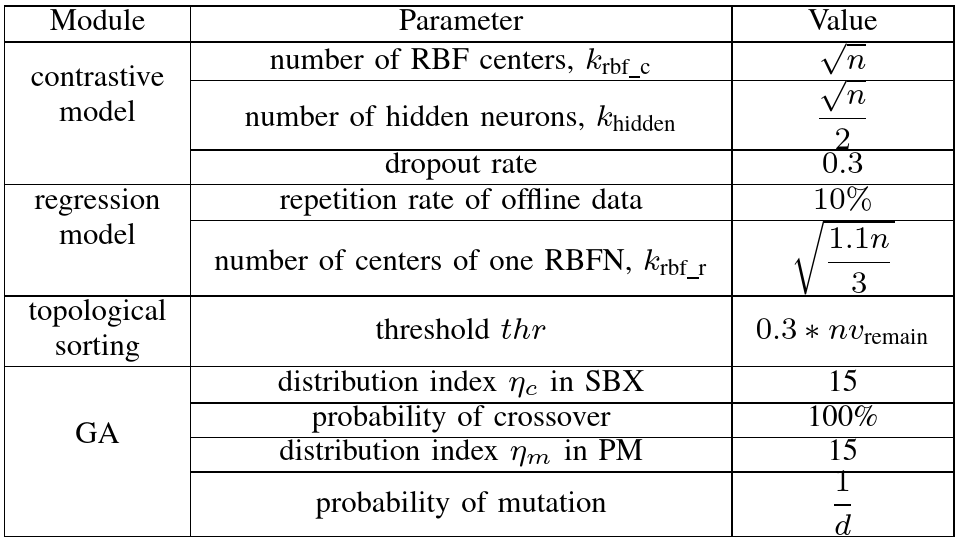
\includegraphics[width=1\textwidth]{./table/figure.png}
            \end{table}
        \end{column}
    \end{columns}
    \hspace{2em} You take a screenshot, and throw the picture into the table environment, such as the table on the right.
\end{frame}

\subsection{Equation}
\begin{frame}
    \frametitle{Equation}
    \begin{block}{Interline Formula}
        \begin{equation}
            \label{eq:example}
            a_n = a_{n-1} + 1
        \end{equation}
    \end{block}
    \begin{block}{Inline Formula}
        This is a simple arithmetic progression formula $a_n = a_{n-1} + 1$.
    \end{block}
\end{frame}

\section{Beamer Reltative}

\subsection{Environment}

\begin{frame}
    \frametitle{block}
    \begin{block}{title}
        \hspace{2em} The content of block.
        You can use hpsace\{2em\} to indent two characters at the beginning of the line if the sentence is long.
    \end{block}
\end{frame}
\begin{frame}
    \frametitle{Abstract}
    \begin{abstract}
        The content of the abstract.
    \end{abstract}
\end{frame}
\begin{frame}[allowframebreaks]
    \frametitle{Math}
    \begin{theorem}[title]
        body
    \end{theorem}
    \begin{lemma}[title]
        body
    \end{lemma}
    \begin{proof}[proof (title).]
        body
    \end{proof}
    \begin{corollary}[title]
        body
    \end{corollary}
    \begin{example}[title]
        body
    \end{example}
    \begin{definition}[title]
        body
    \end{definition}
\end{frame}

\begin{frame}
    \frametitle{alertblock}
    \begin{alertblock}{title}
        body
    \end{alertblock}
\end{frame}

\subsection{Columns}

\begin{frame}
    \frametitle{Columns}
    \begin{columns}
        \column{0.7\textwidth}
        The left side takes up 0.7 width.
        \column{0.3\textwidth}
        The right side takes up 0.3 width.
    \end{columns}
\end{frame}

\subsection{Footnote}

\begin{frame}
    \frametitle{Footnote on Signle Column}
    \hspace{2em} It is a simple \LaTeX~Beamer template for English.
    Please give me a start on Github \footnote{
        \url{https://github.com/h-hg}
    } if it helps you.

    \hspace{2em} Of course, footnotes can also refer to papers \footfullcite{he2016deep}.
\end{frame}

\begin{frame}
    \frametitle{Footnote on Multiple Columns}
    \begin{columns}
        \begin{column}{0.5\textwidth}
            \hspace{2em} Footnotes will not be displayed at the bottom of the page by default in the case of multiple columns,such as \footnote{the default footnote position of multiple columns}.

            \hspace{2em} Citations for papers \footfullcite{he2016deep} are similar.
        \end{column}
        \begin{column}{0.5\textwidth}
            \hspace{2em} However, it can be solved with a [frame], e.g. \footnote[frame]{footntoe with [frame]}.

            \hspace{2em} The citation of the paper \footnote[frame]{\fullcite{he2016deep}} can be achieved with fullcite.
        \end{column}
    \end{columns}
\end{frame}

\section{Others}

\subsection{Highlight}

\begin{frame}
    \frametitle{Short Codes}
    \inputminted[linenos]{cpp}{./code/demo.cpp}
    \hspace{2em} You can choose one of the following two methods if the code is long.
\end{frame}

\begin{frame}
    \frametitle{Two Columns}
    One is achieved through the multicols package and changing the font size of the code to put it on the same page of PPT.
    \begin{multicols}{2}
        \inputminted[linenos,fontsize=\scriptsize]{cpp}{./code/quicksort.cpp}
    \end{multicols}
\end{frame}

\begin{frame}[allowframebreaks]
    \frametitle{Multiple Pages}
    Another is achieved by allowing the code to span multiple PPT pages.
    \inputminted[linenos]{cpp}{./code/quicksort.cpp}
\end{frame}

\subsection{Pseudo-code}

\begin{frame}[allowframebreaks]
    \frametitle{Pseudo-code}
    \begin{algorithm}[H]
        \scriptsize
        \caption{KahnAlgorithm}
        \label{algo:kaha}
        \begin{algorithmic}[1]
    \REQUIRE Graph $G(\mathbb{V}, \mathbb{E})$
    \ENSURE Sequence $L$
    \STATE $L \leftarrow$ an empty sequence
    \STATE $Q \leftarrow$ the vertices whose indegree is zero
    \WHILE{$Q$ is not empty}
        \STATE $u \leftarrow$ remove the top node of $Q$
        \STATE add $u$ to $L$
        \FOR{each node $v$ with an edge $e$ from $u$ to $v$}
            \STATE remove edge $e$ from graph $G$
            \IF{indegree of $v$ is $0$}
                \STATE push $v$ to $Q$
            \ENDIF
        \ENDFOR
    \ENDWHILE
    \RETURN $L$
\end{algorithmic}
    \end{algorithm}
    \begin{columns}
        \begin{column}{0.65\textwidth}
            \begin{algorithm}[H]
                \scriptsize
                \caption{Framework}
                \label{aglo:figure}
                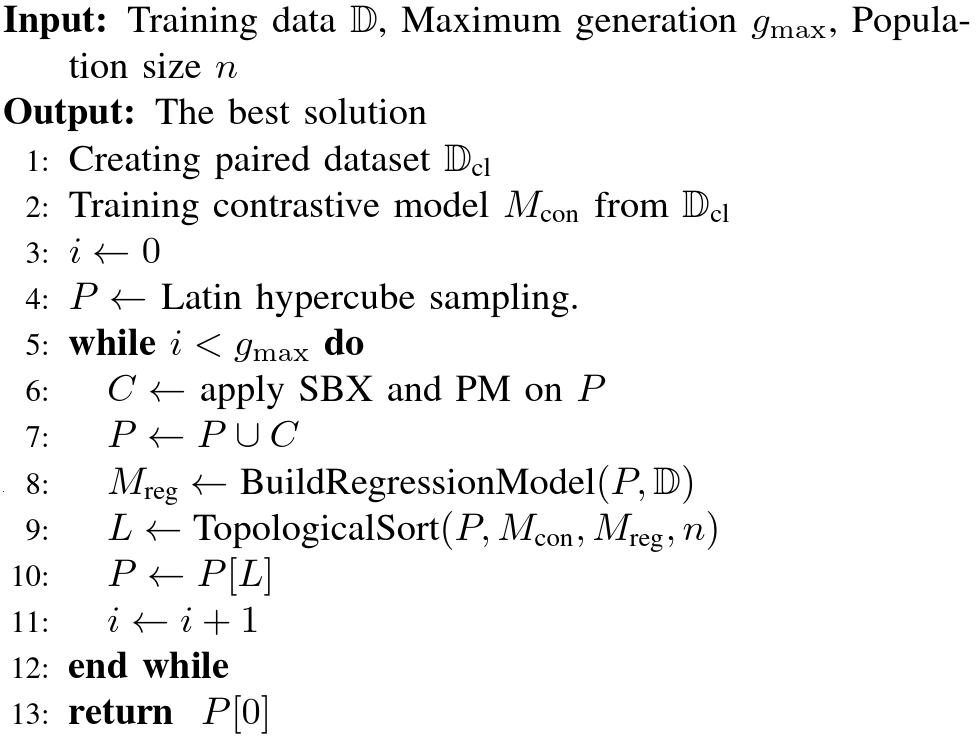
\includegraphics[width=\textwidth]{./algo/figure.png}
            \end{algorithm}
        \end{column}
    \end{columns}
    \hspace{2em} You take a screenshot, and throw the picture into the algorithm environment, such as the algorithm aboved.
\end{frame}


\section*{Reference}
\begin{frame}[allowframebreaks]
    \frametitle{Reference}
    \printbibliography
\end{frame}
  
\section*{Over}
\begin{frame}{}
    \centering
    \huge
    Thanks for your listening!
\end{frame}

\end{document}